% ==========================================
% BAB II STUDI LITERATUR
% ==========================================
\chapter{STUDI LITERATUR}
\label{chap:studi-literatur}
% \section{Penulisan Gambar, Tabel, Rumus, dan Kode}
% \lipsum[1]

\section{Mahasiswa, Kolaborasi, dan Pengembangan Diri}
Menurut \textcite{novitaCOLLABORATIVELEARNINGMANIFESTATION2020}, Kolaborasi antar mahasiswa merupakan fondasi utama dalam pendidikan tinggi modern yang mendukung pengembangan kompetensi abad ke-21, seperti berpikir kritis, kreativitas, komunikasi, dan kolaborasi (4C), sebagaimana diuraikan dalam kerangka Partnership for 21st Century Skills yang menekankan keterampilan ini untuk kesiapan kerja di era digital. Teori sosial konstruktivisme Lev Vygotsky (1978) menjelaskan bahwa interaksi sosial melalui \textit{Zone of Proximal Development} (ZPD) memungkinkan mahasiswa mencapai potensi perkembangan yang lebih tinggi dengan bantuan rekan sebaya, di mana kolaborasi memfasilitasi pertukaran pengetahuan dan pembentukan pemahaman baru yang lebih mendalam. Dalam konteks perguruan tinggi Indonesia, penelitian menunjukkan bahwa pembelajaran kolaboratif melalui proyek berbasis tim meningkatkan keterampilan kerja sama mahasiswa, yang berkontribusi langsung terhadap pengembangan diri seperti inovasi ide dan adaptabilitas profesional.​

Kolaborasi tidak hanya memperkaya aspek kognitif, tetapi juga membangun pengembangan diri holistik melalui pengelolaan dinamika kelompok, di mana mahasiswa belajar bernegosiasi, berbagi tanggung jawab, dan mengelola konflik untuk mencapai tujuan bersama. Menurut \textcite{sansonePromoting21stCentury2018}, aktivitas kolaboratif seperti diskusi kelompok dan proyek bersama meningkatkan rasa percaya diri serta kemampuan adaptif mahasiswa terhadap tantangan lingkungan kerja yang kompleks. Hal ini selaras dengan temuan bahwa kolaborasi mendorong diversifikasi perspektif, sehingga mahasiswa tidak terbatas pada homophily pertemanan sempit, melainkan terbuka terhadap paparan keterampilan baru yang esensial untuk kolaborasi.​​

Pengembangan diri melalui kolaborasi mahasiswa juga tercermin dalam peningkatan literasi digital dan keterampilan sosial, di mana interaksi tim menghasilkan ide solutif dan kreatif yang mendukung pencapaian hasil belajar optimal. Menurut perspektif Lev Vygotsky (1978), proses ini bersifat sosial dan kontekstual, sehingga relevan dengan aplikasi kolaborasi mahasiswa yang menampilkan profil rekan potensial berdasarkan keselarasan atribut. Dengan demikian, kolaborasi menjadi katalisator pengembangan diri yang berkelanjutan, mempersiapkan mahasiswa menghadapi tuntutan industri yang menuntut kerja tim lintas disiplin.

\section{Tantangan Mencari Partner Kolaborasi Mahasiswa}
Meskipun kolaborasi dan kerja kelompok menjadi bagian penting dalam pendidikan tinggi karena manfaatnya dalam pengembangan \textit{soft-skills}, kreativitas, dan hasil belajar yang lebih baik, banyak studi menunjukkan bahwa proses kolaborasi mahasiswa tidak selalu berjalan mulus. Berbagai tantangan dapat menghambat mahasiswa dalam menemukan partner atau tim yang cocok, yang pada gilirannya dapat menurunkan kualitas kerja kelompok, motivasi, dan hasil kolaborasi. Di bawah ini dijabarkan sejumlah tantangan utama berdasarkan studi literatur.
\begin{enumerate}
\item {Partisipasi tidak merata}

Banyak mahasiswa melaporkan bahwa dalam kerja kelompok, kontribusi tidak terbagi rata: sebagian anggota melakukan sebagian besar pekerjaan sementara yang lain kurang aktif (\textit{free-rider}). Studi oleh \textcite{changWhenGroupWork2018} menunjukkan bahwa ketidaksetaraan kontribusi ini menjadi keluhan utama dalam kerja kelompok di perguruan tinggi. Hal serupa ditemukan dalam literatur “challenges in group work” yang menyebutkan “\textit{low and uneven participation by students}” sebagai masalah signifikan dalam proyek kelompok, terutama pada proyek daring. Ketimpangan kontribusi ini tidak hanya merusak dinamika kelompok tetapi juga memunculkan ketidakadilan persepsi terhadap beban kerja yang akhirnya membuat mahasiswa enggan berkolaborasi ulang.

\item{Kesulitan komunikasi dan koordinasi}

Kolaborasi menuntut komunikasi yang efektif dan koordinasi antar anggota. Namun, banyak penelitian menunjukkan bahwa komunikasi buruk, baik karena kurangnya struktur, ketidakjelasan peran, atau perbedaan ekspektasi menjadi hambatan besar. Dalam penelitian \textcite{pangSociallyChallengedCollaborative2018} pada mahasiswa, tim dengan komunikasi buruk sering gagal mencapai hasil optimal. Selain itu, perubahan lingkungan (misalnya pembelajaran daring) memperburuk tantangan ini; siswa melaporkan penurunan kepuasan, motivasi, dan efektivitas kerja kelompok ketika kolaborasi dilakukan secara \textit{online}.

\item{Perbedaan minat, komitmen, gaya kerja, beban aktivitas}

Kelompok mahasiswa lazimnya beranggotakan individu dengan latar belakang, minat, motivasi, serta tingkat komitmen yang beragam, sehingga potensi gesekan muncul sejak tahap pemilihan rekan hingga pelaksanaan kerja tim. Literatur tentang kerja kelompok menunjukkan bahwa perbedaan ekspektasi peran, standar kontribusi, dan preferensi gaya kerja kerap memicu perilaku “pemalasan sosial” (\textit{free‑riding}) dan persepsi ketidakadilan dalam distribusi beban, terutama ketika kohesivitas tim rendah dan tujuan tidak terkomunikasikan dengan jelas. Lebih jauh, resistensi mahasiswa terhadap kerja kelompok juga dipengaruhi faktor psikologis seperti rasa penguasaan diri belajar yang terbatas dan resistensi terhadap perubahan yang berdampak pada komitmen dan koordinasi tugas \textcite{sulisRESISTANCECHANGEMAHASISWA2020}. Dalam konteks pengalaman belajar sehari‑hari, temuan kualitatif menandai bahwa mengatur kolaborasi dengan rekan yang beragam sering menjadi tantangan utama mahasiswa, mulai dari pembagian peran, manajemen waktu, hingga menjaga konsistensi standar kualitas. 

\item{Ketidakpastian dalam membentuk tim karena tidak ada mekanisme pencocokan}

Banyak mahasiswa mengandalkan pertemanan, kebetulan, atau koneksi sosial terbatas ketika mencari teman kolaborasi. Hal ini menyebabkan kecenderungan “homogenitas lingkaran” sehingga sulit untuk menemukan rekan dengan minat atau skill spesifik yang dibutuhkan proyek. Studi literatur \textcite{darbyMakingGroupWork} berpendapat bahwa tanpa struktur atau sistem yang mendukung, proses formasi tim bisa random dan kurang optimal. Khususnya dalam proyek daring atau lintas kampus, hambatan ini makin terasa karena kurangnya informasi tentang calon anggota, kesulitan penilaian kesesuaian, dan komunikasi terbatas.

\item{Konflik interpersonal, perbedaan ekspektasi, dan ketidakjelasan peran}

Konflik tim seperti perbedaan komitmen, ekspektasi hasil, ketidakjelasan pembagian tugas, atau kurangnya transparansi sering terjadi. Penelitian \textcite{omodanAddressingPotentialConflict2023} menunjukkan bahwa konflik dan perasaan tidak adil akibat kontribusi yang timpang atau komitmen berbeda mengurangi motivasi dan efektivitas tim. Konflik interpersonal dan dinamika sosial ini mempersulit kerja sama yang produktif.

\item{Kesulitan dalam mencari partner baru di luar lingkaran pertemanan}

Banyak mahasiswa enggan mencari partner di luar teman dekat karena ketidakpastian, tidak mengenal karakteristik orang lain, tidak tahu skill/komitmen, dan takut risiko kerja buruk. Hasil penelitian \textcite{pradinaDampakKohesivitasKelompok2024} menunjukkan resistensi terhadap kerja kelompok jika partner dianggap asing atau tidak dapat dipercaya. Hal ini memunculkan “tembok sosial” yang membuat kolaborasi sulit diperluas padahal banyak proyek membutuhkan tim dengan keahlian atau minat khusus.
\end{enumerate}

\section{\textit{Software Development Life Cycle} (SDLC)}
\textit{Software Development Life Cycle} (SDLC) merupakan kerangka proses yang digunakan untuk mengembangkan perangkat lunak secara sistematis, terstruktur, dan dapat dikendalikan. Menurut \textcite{sommervilleSoftwareEngineering2016}, SDLC memastikan bahwa setiap tahapan pengembangan mulai dari perumusan kebutuhan hingga pemeliharaan dilakukan secara konsisten untuk menghasilkan sistem yang memenuhi kebutuhan pengguna dan memiliki kualitas yang dapat dipertanggungjawabkan. SDLC secara umum mencakup beberapa fase inti seperti analisis kebutuhan, perancangan sistem, implementasi, pengujian, serta pemeliharaan. Pendekatan ini penting karena pengembangan perangkat lunak bukan hanya sekedar membangun fitur, tetapi juga mengelola risiko, mendokumentasikan keputusan, dan menjaga agar hasil akhir tetap sesuai dengan tujuan awal. 

\subsection{\textit{Waterfall Model}}
Model \textit{Waterfall} adalah salah satu pendekatan SDLC paling klasik dan banyak digunakan dalam proyek yang memiliki kebutuhan stabil serta ruang lingkup yang terdefinisi dengan jelas. \textcite{sommervilleSoftwareEngineering2016} menjelaskan bahwa \textit{Waterfall} bekerja secara berurutan (sekuensial), di mana setiap fase harus diselesaikan sebelum beralih ke fase berikutnya. Pendekatan linear ini memberikan struktur yang kuat, dokumentasi yang lengkap, serta kontrol yang baik terhadap alur pengembangan.

\section{Sistem Rekomendasi}
Sistem rekomendasi merupakan komponen penting dalam banyak aplikasi modern yang membantu pengguna menemukan informasi atau entitas yang relevan dari sekian banyak pilihan yang tersedia. Menurut \textcite{ricciIntroductionRecommenderSystems2011}, sistem rekomendasi bekerja dengan melakukan penyaringan informasi (\textit{information filtering}) dan menampilkan rekomendasi yang sesuai dengan kebutuhan atau preferensi pengguna. Sistem ini berkembang luas dalam berbagai domain, mulai dari \textit{e-commerce}, media, pendidikan, hingga platform kolaborasi digital.

Secara umum, \textcite{adomaviciusNextGenerationRecommender2005} mengelompokkan pendekatan sistem rekomendasi ke dalam tiga kategori utama: \textit{content-based}, \textit{collaborative filtering}, dan \textit{knowledge-based}. Pendekatan \textit{content-based} memberikan rekomendasi berdasarkan kesamaan karakteristik item dengan preferensi pengguna. \textit{Collaborative filtering} menggunakan pola perilaku dan kesamaan antar pengguna. Namun, kedua pendekatan tersebut kurang sesuai untuk konteks \textit{people-to-people matching}, terutama ketika pengguna belum memiliki riwayat interaksi atau ketika penilaian kecocokan membutuhkan pemahaman mendalam terhadap atribut profil pengguna.

Dalam konteks pencarian partner kolaborasi mahasiswa, pendekatan \textit{knowledge-based recommendation} menjadi lebih relevan. Pendekatan ini memanfaatkan pengetahuan eksplisit mengenai atribut pengguna, seperti minat, kemampuan, atau preferensi kerja, untuk menentukan tingkat kecocokan antara dua entitas. Sistem kemudian dapat menghasilkan peringkat rekomendasi berdasarkan kesesuaian atribut tersebut. Pendekatan ini lebih transparan, mudah dijelaskan, dan sesuai untuk domain yang membutuhkan rekomendasi berbasis profil pengguna, bukan perilaku historis.

Dengan demikian, sistem rekomendasi dalam tugas akhir ini berfungsi sebagai mekanisme untuk membantu mahasiswa menemukan calon partner kolaborasi yang relevan berdasarkan kesesuaian atribut pengguna. Sistem ini menjadi dasar bagi pengembangan fitur \textit{People-to-People} yang menampilkan profil mahasiswa secara terurut sesuai tingkat kecocokan, sehingga dapat mengurangi tantangan dalam proses pencarian rekan kolaborasi.

\subsection{\textit{Rule Based Matching}}
\textit{Rule-based matching} merupakan pendekatan pencocokan yang menentukan kesesuaian antara dua entitas berdasarkan seperangkat aturan atau kriteria yang telah didefinisikan sebelumnya. Pendekatan ini bekerja dengan cara memeriksa atribut-atribut tertentu dari entitas yang akan dicocokkan, kemudian memberikan evaluasi kesesuaian berdasarkan logika yang eksplisit, seperti \textit{if–then rules}, pembobotan atribut, atau penilaian berbasis skor. Menurut \textcite{burkeKnowledgebasedRecommenderSystems}, sistem rekomendasi berbasis pengetahuan (\textit{knowledge-based recommendation}) umumnya menggunakan aturan untuk menilai apakah suatu item atau entitas memenuhi kebutuhan pengguna, sehingga menghasilkan rekomendasi yang dapat dijelaskan dan dipertanggungjawabkan secara logis. Dengan demikian, \textit{rule-based} matching termasuk dalam kategori \textit{knowledge-based system} karena menggunakan pengetahuan domain untuk menghasilkan rekomendasi yang relevan.

\textit{Rule-based matching} banyak digunakan dalam situasi di mana proses pencocokan tidak dapat mengandalkan data historis, atau ketika kesesuaian perlu diukur secara eksplisit menggunakan atribut yang jelas, misalnya minat, kemampuan, pengalaman, atau preferensi kerja. \textcite{adomaviciusNextGenerationRecommender2005} menjelaskan bahwa pendekatan semacam ini sangat berguna untuk mengatasi permasalahan \textit{cold-start} pada sistem rekomendasi, yaitu kondisi ketika pengguna belum memiliki riwayat interaksi sehingga metode berbasis perilaku seperti \textit{collaborative filtering} tidak dapat diterapkan. Dengan menggunakan aturan dan bobot atribut tertentu, sistem dapat menghasilkan rekomendasi meskipun data perilaku pengguna masih sangat minim.

Pendekatan \textit{rule-based} juga memiliki keunggulan dari sisi transparansi dan interpretabilitas. Karena aturan pencocokan didefinisikan secara eksplisit, pengguna dan pengembang dapat memahami bagaimana rekomendasi dihasilkan, apakah suatu profil dinilai cocok atau tidak, serta atribut mana yang berpengaruh dalam proses pemeringkatan. Hal ini membuat \textit{rule-based matching} sangat sesuai dalam konteks \textit{people-to-people recommendation}, di mana pencocokan perlu mempertimbangkan atribut personal seperti minat akademik, kemampuan teknis, gaya kerja, atau komitmen waktu. Aturan ini dapat digunakan untuk menghitung tingkat kesesuaian antara dua profil dan menyusun urutan rekomendasi secara terstruktur, yang kemudian ditampilkan pada fitur \textit{People-to-People}.

Dengan demikian, \textit{rule-based matching} memberikan fondasi yang kuat untuk membangun mekanisme rekomendasi yang terarah dan dapat dijelaskan. Pendekatan ini menjadi landasan bagi pengembangan model \textit{affinity} pada tugas akhir ini, di mana atribut-atribut pengguna akan diberi bobot tertentu sehingga keselarasan antarprofil dapat dinilai dan diurutkan secara kuantitatif.

\subsection{\textit{Affinity based matching}}
\textit{Affinity-based matching} merupakan pendekatan pencocokan yang menilai tingkat keselarasan antara dua entitas berdasarkan sejumlah atribut yang mewakili karakteristik, minat, kemampuan, atau preferensi masing-masing pihak. Konsep \textit{affinity} pada dasarnya merujuk pada tingkat kedekatan atau kecocokan yang dapat dihitung secara kuantitatif menggunakan model pembobotan atribut dan perhitungan skor kesesuaian. Dalam konteks sistem rekomendasi, pendekatan ini digunakan untuk menyusun peringkat rekomendasi berdasarkan skor keselarasan, sehingga entitas dengan kecocokan tertinggi dapat ditampilkan lebih dahulu \textcite{burkeKnowledgebasedRecommenderSystems}.

Berbeda dengan \textit{collaborative filtering} yang mengandalkan pola perilaku pengguna, \textit{affinity-based matching} mengandalkan pengetahuan eksplisit tentang atribut suatu entitas. Oleh karena itu, pendekatan ini termasuk dalam kategori \textit{knowledge-based recommendation}, yaitu sistem rekomendasi yang menghasilkan output berdasarkan penalaran atas karakteristik pengguna dan objek yang direkomendasikan. Pendekatan ini sangat relevan untuk domain yang membutuhkan pemahaman mendalam mengenai kecocokan antar entitas, seperti pencarian partner kolaborasi mahasiswa, karena kesesuaian tidak dapat ditentukan hanya dari riwayat interaksi, melainkan harus mempertimbangkan atribut personal dan preferensi kerja. \textit{Affinity-based} matching umumnya bekerja melalui proses berikut:
\begin{enumerate}
\item {Identifikasi atribut relevan seperti minat, kemampuan teknis, pengalaman proyek, preferensi gaya kerja, atau komitmen waktu.} 
\item {Pembobotan atribut berdasarkan tingkat pengaruhnya terhadap kecocokan.}
\item {Perhitungan \textit{skor affinity}, yaitu nilai yang menggambarkan seberapa cocok dua profil satu sama lain.}
\end{enumerate}
Pemeringkatan rekomendasi, di mana profil dengan skor tertinggi ditampilkan lebih dahulu dalam daftar rekomendasi. Model pembobotan seperti \textit{weighted-sum model} atau \textit{similarity scoring} sering digunakan untuk menghitung affinity karena sifatnya yang transparan, mudah dijelaskan, dan dapat dikendalikan oleh pengembang. Model seperti ini juga banyak digunakan dalam penelitian sistem rekomendasi berbasis pengetahuan untuk menghasilkan rekomendasi yang konsisten dan dapat dipertanggungjawabkan \textcite{adomaviciusNextGenerationRecommender2005}.

Dalam konteks pencarian rekan kolaborasi mahasiswa, \textit{affinity-based matching} menawarkan beberapa keunggulan. Pertama, pendekatan ini mampu mengatasi keterbatasan informasi pada pengguna baru (\textit{cold start}) karena tidak membutuhkan riwayat perilaku. Kedua, proses pencocokan dapat disesuaikan dengan kebutuhan spesifik mahasiswa, misalnya minat bidang tertentu, kemampuan teknis tertentu, atau preferensi kerja. Ketiga, model \textit{affinity} memberikan fleksibilitas untuk menampilkan hasil dalam bentuk fitur  People-to-People, yaitu alur rekomendasi berbasis peringkat yang menyerupai tampilan aplikasi sosial modern.

Pendekatan \textit{affinity} ini mendukung tujuan tugas akhir, yakni menyediakan mekanisme rekomendasi partner kolaborasi yang relevan, terarah, dan dapat dijelaskan secara logis. Hasil perhitungan \textit{affinity} menjadi dasar bagi urutan rekomendasi pada \textit{feed}, sehingga mahasiswa dapat menemukan calon rekan kolaborasi yang paling sesuai dengan karakteristik dan preferensi mereka.

\section{\textit{User Centered Design (UCD)}}
\textit{User-Centered Design} (UCD) merupakan pendekatan perancangan yang menempatkan pengguna sebagai pusat dalam setiap tahap pengembangan sistem. Prinsip utama UCD adalah bahwa sebuah sistem akan lebih efektif dan mudah digunakan apabila dirancang berdasarkan pemahaman terhadap kebutuhan, karakteristik, lingkungan, dan tujuan pengguna. Standar internasional ISO 9241-210:2010 mendefinisikan UCD sebagai \textit{human-centred design}, yaitu proses iteratif yang memastikan solusi akhir benar-benar sesuai dengan konteks penggunaan dan mendukung pengalaman pengguna secara optimal.
\begin{figure}[h] % pilihan opsi yang disarankan: t = top, b = bottom, h = here
	\centering
  \captionsetup{justification=centering}
    	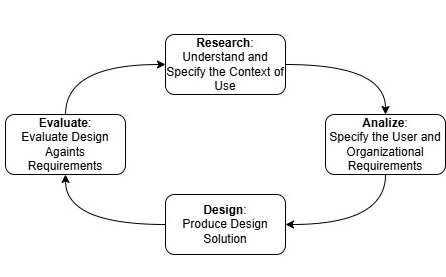
\includegraphics[width=0.7\textwidth]{image/UCD.jpg}
	\caption{Siklus \textit{User-Centered Design} berdasarkan ISO 9241-210}
	\label{gambar:UCD}
\end{figure}
Menurut \textcite{rogers2015interaction}, UCD melibatkan siklus berulang yang mencakup pemahaman konteks penggunaan, perumusan kebutuhan pengguna, pengembangan solusi desain, serta evaluasi desain berdasarkan umpan balik pengguna. Pendekatan ini berbeda dengan metode perancangan tradisional karena keputusan desain tidak hanya berasal dari asumsi pengembang, melainkan dari hasil riset pengguna (user research) yang terstruktur. Dengan demikian, UCD membantu memastikan bahwa sistem yang dikembangkan tidak hanya fungsional tetapi juga \textit{usable, meaningfully relevant}, dan mudah dipahami. Sesuai standar ISO 9241-210, terdapat empat aktivitas utama UCD yang saling terhubung dan dilakukan secara iteratif:
\begin{enumerate}
\item {Memahami konteks penggunaan}

Melibatkan identifikasi pengguna, tugas pengguna, tujuan, motivasi, dan lingkungan operasional. Pada tugas akhir ini, konteks ditentukan melalui studi literatur dan pengumpulan data melalui kuesioner mengenai pengalaman mahasiswa dalam mencari partner kolaborasi.

\item {Menentukan kebutuhan pengguna dan kebutuhan sistem}

Hasil analisis pengguna diterjemahkan menjadi kebutuhan fungsional dan non-fungsional. Misalnya, kebutuhan untuk menampilkan profil mahasiswa secara ringkas, relevan, serta dilengkapi atribut minat, kemampuan, dan preferensi kerja.

\item {Menghasilkan solusi desain}

Tahap ini mencakup pembuatan user flow, wireframe, dan rancangan antarmuka fitur \textit{People-to-People}. Proses ini dilakukan secara iteratif dan dapat melibatkan prototipe rendah (\textit{low fidelity}) sebelum dikembangkan menjadi desain antarmuka akhir.

\item {Evaluasi terhadap solusi desain}

Evaluasi dilakukan untuk memastikan bahwa desain memenuhi kebutuhan pengguna, misalnya menggunakan \textit{expert review}, \textit{heuristic evaluation}, atau uji coba terbatas. Hasil evaluasi digunakan untuk memperbaiki desain pada iterasi berikutnya.

\end{enumerate}



